% !TEX root = ../RAN_MFA.tex

\bexo
Let consider the following transformation\\
 \begin{center}
 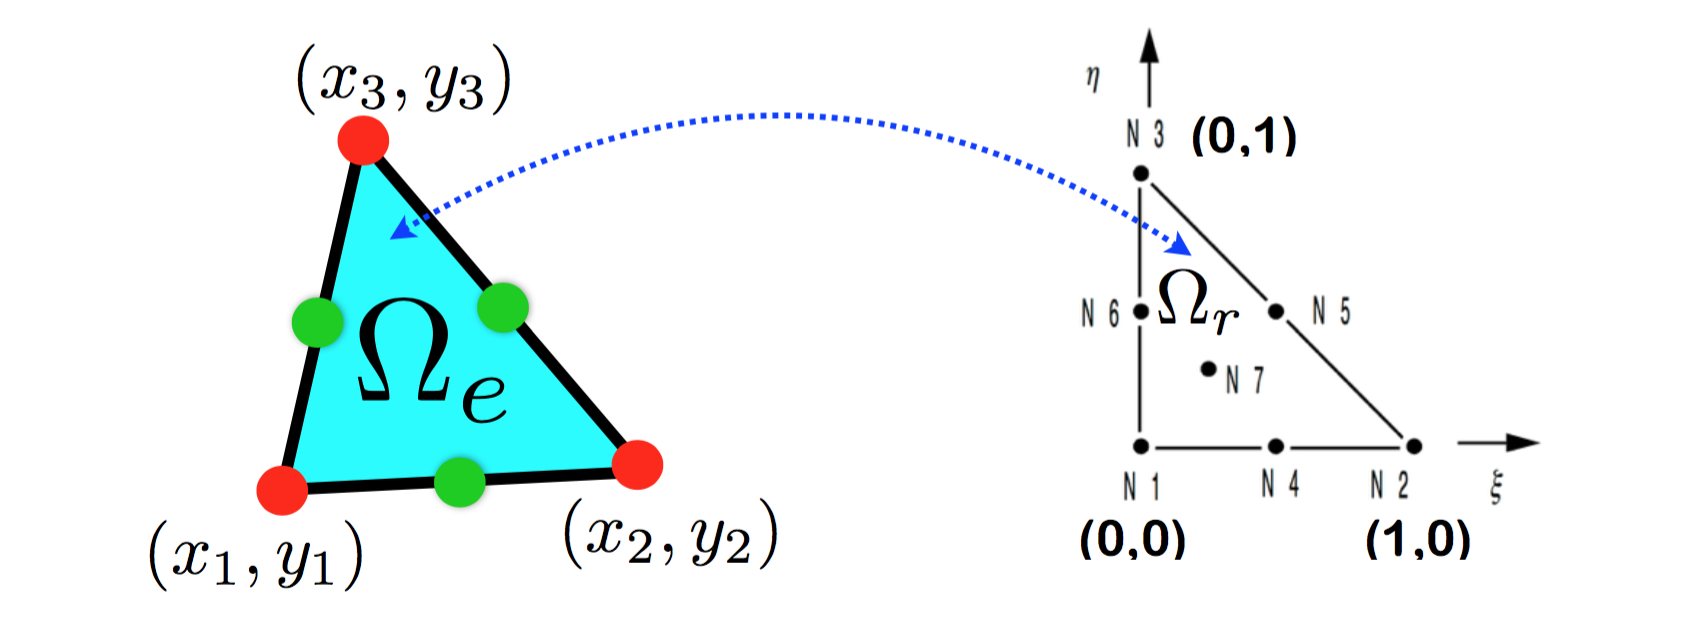
\includegraphics[width=0.7\textwidth]{../TeX_Files/Calculus/reference_element.png}
 \end{center}
 A given triangle $\mc{T}$ of vertices $(x_1,y_1)$, $(x_2,y_2)$ and $(x_3,y_3)$ is transformed into an isosceles rectangle triangle $\mc{T}_{ref}$. A point of coordinates $(x,y)$ in $\mc{T}$ is associated to a point $(\xi,\eta)$ in $\mc{T}_{ref}$. The transformation is then as follows:
 \begin{equation}
 f:\left\{
 \begin{array}{ccc}
 	\mc{T}_{ref} &\longrightarrow &\mc{T}\\
 	\begin{Bmatrix}
 		\xi\\\eta
 	\end{Bmatrix}
 	&\mapsto & 	\begin{Bmatrix}
 		x(\xi,\eta)\\
 		y(\xi,\eta)
 		 	\end{Bmatrix}
 \end{array}
 \right.	
 \end{equation}
This transformation relates the vertices as follows
\begin{align}
	f(0,0)&=(x_1,y_1)\\
	f(1,0)&=(x_2,y_2)\\
	f(0,1)&=(x_3,y_3)\\
\end{align} 
 

 \begin{itemize}
 	\item What is the expression of matrix $\{\bs{\Phi}(\xi,\eta)\}$ so that 
 \begin{equation}
 	\begin{Bmatrix}
 		x(\xi,\eta)\\
 		y(\xi,\eta)
 		 	\end{Bmatrix}=\begin{bmatrix}
 		 		x_1 & x_2 & x_3\\
 		 		y_1 & y_2 & y_3
 		 	\end{bmatrix}\{\bs{\Phi}(\xi,\eta)\}
 \end{equation}
 Compute the Jacobian Matrix $J$ of transformation $f$. $J$ is defined as 
 \begin{equation}
 	J=\begin{bmatrix}
 		\dfrac{\p x}{\p \xi} & \dfrac{\p x}{\p \eta}\\
 		\dfrac{\p y}{\p \xi} & \dfrac{\p y}{\p \eta}
 	\end{bmatrix}
 \end{equation} 
 \end{itemize}
  
\eexo

\solution{
\begin{equation}
	\{\bs{\Phi}(\xi,\eta)\}=\begin{Bmatrix}
		1-\eta-\xi \\ \xi \\ \eta
	\end{Bmatrix}
\end{equation}

 \begin{equation}
 	J=\begin{bmatrix}
 		-x_1+x_2 & -x_1+x_3\\
 		-y_1+y_2 & -y_1+y_3
 	\end{bmatrix}
 \end{equation} 


}